\documentclass[UTF8]{ctexart}
\usepackage[paper=a4paper,dvips,top=2.5cm,left=2.8cm,right=2.8cm,foot=1cm,bottom=3.2cm]{geometry}
\usepackage{fancyhdr}
\usepackage{indentfirst}
\usepackage{enumerate}
\usepackage{clrscode}
\usepackage{listings}
\usepackage{amsmath}
\usepackage{amstext}
\lstset{language=Matlab}%代码语言使用的是matlab
\lstset{breaklines}%自动将长的代码行换行排版
\lstset{extendedchars=false}%解决代码跨页时,章节标题,页眉等汉字不显示的问题
\usepackage{graphicx}
\usepackage[colorlinks,linkcolor=blue,urlcolor = blue]{hyperref}
\DeclareGraphicsExtensions{.eps,.ps,.jpg,.bmp}
\pagestyle{plain}
\begin{document}
\par 尊敬的吴老师,您好
\newline
\par
我想先用一个例子,简要介绍一下训练过程,以及论文中一处不合理的地方。
\begin{figure}[h!]
    \centering
    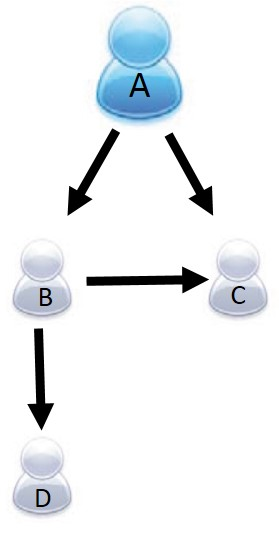
\includegraphics[width=2cm]{social_influence.jpg}
    \caption{微博用户网络示例}
    \label{fig-sample}
\end{figure}
\par 如图1所示(黑色箭头表示“关注”关系),假设对于一条微博$m$,它的转发链为
\begin{equation*}
\left \{ A,B,C,D \right \}
\end{equation*}
据此,我们可以得到每个用户的上下文链,如表1所示。
\begin{table}[!hbp]
\centering
\begin{tabular}{|c|c|c|c|c|}
\hline
\hline
 用户 &  $i=1$ &  $i=2$ &  $i=3$ &  $i=4$ \\
\hline
 A &  $\left \{  \right \}$ &  $\left \{  \right \}$ & $\left \{  \right \}$  &  $\left \{  \right \} $\\
\hline
 B &  $\left \{ A \right \}$ &  $\left \{ A \right \}$ &  $\left \{ A \right \}$ &  $\left \{ A \right \}$ \\
\hline
 C &  $\left \{ A \right \}$ &  $\left \{ A,B \right \}$ &  $\left \{ A,B \right \}$ &  $\left \{ A,C \right \}$ \\
\hline
 D &  $\left \{  \right \}$ &  $\left \{ B \right \}$ &  $\left \{ B \right \}$ &  $\left \{ B \right \}$ \\
 \hline
\hline
\end{tabular}
\caption{用户上下文链$D_{v,i}^{m}$}
\end{table}
\par 此时的状态向量为
\begin{equation*}
\begin{matrix}
\begin{aligned}
z_{A}^{m} = \left [ 1,1,1,1,1 \right ]^{T} \\
z_{B}^{m} = \left [ 0,1,1,1,1 \right ]^{T} \\
z_{C}^{m} = \left [ 0,0,1,1,1 \right ]^{T} \\
z_{D}^{m} = \left [ 0,0,0,1,1 \right ]^{T} \\
\end{aligned}
\end{matrix}
\end{equation*}
\par 接下来需要求解$P(z_{v}\mid \delta)$,我们以$P(z_{B}\mid \delta)$作为示例。
\par 由于$B$并非微博$m$的始发者,因此
\begin{equation*}
p(z_{B,0}^{m}=0) = 1-p(z_{B,0}^{m}=1) = 1
\end{equation*}
\par 根据$z_{B}^{m} = \left [ 0,1,1,1,1 \right ]^{T} $和$\delta(A,B)=1$(根据图$1$),可以得到
\begin{equation*}
\begin{matrix}

p(z_{B,1}^{m}=1 \mid z_{B,0}^{m}=0,D_{B,1}^{m},\delta) = 1- exp(-\lambda \delta(A,B)\sum _{u\in D_{B,1}^{m}}I_{u}^{T}S_{v})=1-exp(-\lambda I_{A}^{T}S_{v}) \\
p(z_{B,2}^{m}=1 \mid z_{B,1}^{m}=1,D_{B,2}^{m},\delta) = 1 \\
p(z_{B,3}^{m}=1 \mid z_{B,2}^{m}=1,D_{B,3}^{m},\delta) = 1 \\
p(z_{B,4}^{m}=1 \mid z_{B,3}^{m}=1,D_{B,4}^{m},\delta) = 1 

\end{matrix}
\end{equation*}
\par 而$P(z_{B}^{m}\mid \delta) $即为它们相乘的结果,即
\begin{equation*}
P(z_{B}^{m}\mid \delta) = 1-exp(-\lambda I_{A}^{T}S_{v})
\end{equation*}
\par 用户A、C、D状态向量$z_{v}^{m}$的概率的求法与上面类似,最终我们可以得到$L(C)$。当然,我们在训练过程中并不需要计算$L(C)$,只需要计算$\frac{\partial L}{I_{u}}$和$\frac{\partial L}{S_{v}}$,然后利用投影梯度法更新$I$和$S$。不断重复上述过程,直到论文的公式($6$)达到最小值。
\begin{equation*}
L(C) = \prod _{m=1}^{\left | C \right |}\prod _{v \in V}P(z_{v}^{m} \mid \delta)
\end{equation*}
\par 假如我们还有很多微博在图$1$所示的网络中传播,我们不难发现用户的上下文链有大量的重叠。为了避免冗余计算,所以论文中提出了公式($7$),将所有消息的上下文链按用户分组。
\par 总结一下训练过程:
\begin{enumerate}[\indent 1)]
    \item 构建diffusion network,以求解$\delta(u,v)$
    \item 对每一条消息,求解上下文链$D_{v,i}^{m}$,并对用户分组,得到$D_{v,i}$
    \item 对每一条消息,求解状态向量$z_{v,i}$
    \item 按照论文中Algorithm 1计算$I,S$
\end{enumerate}
\subsubsection*{原论文中一个不合理的地方}
\par 论文中的公式($4$)是这样的
\begin{equation*}
p(z_{v,i}^{m}=1 \mid z_{v,i-1}^{m}=0,D_{v,i}^{m},\delta)=1-exp(-\lambda \delta(a_{i}^{m},v)\sum _{u \in D_{v,i}^{m}}I_{u}^{T}S_{v})
\end{equation*}
其中的$\delta(a_{i}^{m},v)$的$a_{i}^{m}$表示消息$m$的转发链中的第$i$个用户,这在真实网络中明显不合理!
\par 举个例子,对于图1,某时刻用户A作为始发者,转发了一条信息$m$,B、C作为粉丝,受到A的影响,也转发了此消息,且B要比C先转发。此时得到的转发链为$\left \{ A,B,C \right \}$。根据公式($4$)计算$p(z_{C,2}^{m}=1 \mid z_{v,1}^{m}=0,D_{v,2}^{m},\delta)$时,公式($4$)中的$\delta(a_{i}^{m},C)$为$\delta(B,C)$。但我们知道C之所以转发信息,是受A的影响,而非B!这样可能造成\textbf{本应属于A的影响力部分的转移到了B身上}。再者,假如B到C之间没有连边,那么$\delta(B,C)=0$,最终导致公式($6$)计算的$L(C)$趋于无穷大。
\par 这可能是作者的笔误,也有可能是我对文章的理解不到位。
\newline
\par \rightline{学生王超民,2016年5月10日}

\end{document}
